\documentclass[tikz,border=2pt]{standalone}
\usepackage{amsmath,amssymb}
\usepackage{tikz}
\usetikzlibrary{arrows.meta}

\begin{document}
% A left inverse undoes f (needs f injective); a right inverse is undone by f (needs f
% surjective); both exist exactly when f is bijective, and then they coincide.
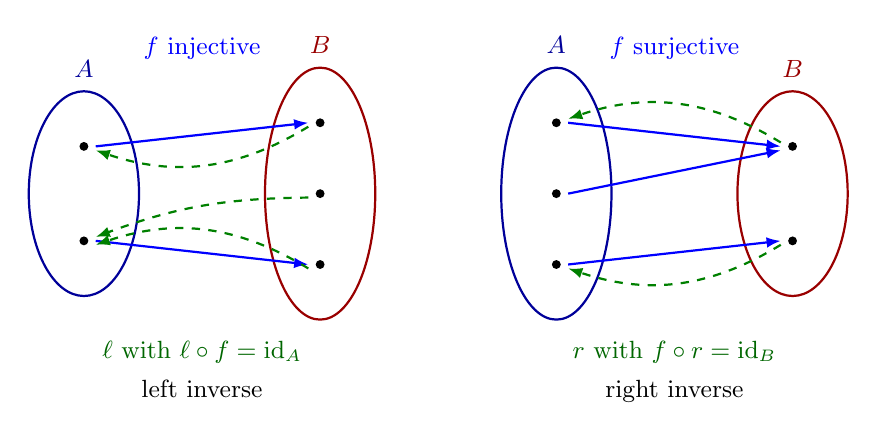
\begin{tikzpicture}[every node/.style={font=\small}, >={Latex[length=1.8mm]}]
	\begin{scope}
		\draw[thick, blue!60!black] (0,0) ellipse (0.7 and 1.3); \node[blue!60!black, anchor=south] at (0,1.35) {$A$};
		\draw[thick, red!60!black] (3,0) ellipse (0.7 and 1.6); \node[red!60!black, anchor=south] at (3,1.65) {$B$};
		\fill (0,0.6) circle (1.6pt); \fill (0,-0.6) circle (1.6pt);
		\fill (3,0.9) circle (1.6pt); \fill (3,0) circle (1.6pt); \fill (3,-0.9) circle (1.6pt);
		\draw[->, blue, thick] (0.15,0.6) -- (2.85,0.9);
		\draw[->, blue, thick] (0.15,-0.6) -- (2.85,-0.9);
		\draw[->, green!50!black, thick, dashed] (2.85,0.85) to[bend left=25] (0.15,0.55);
		\draw[->, green!50!black, thick, dashed] (2.85,-0.95) to[bend right=25] (0.15,-0.65);
		\draw[->, green!50!black, thick, dashed] (2.85,-0.05) to[bend right=10] (0.15,-0.55);
		\node[blue] at (1.5,1.85) {$f$ injective};
		\node[green!40!black, anchor=north] at (1.5,-1.75) {$\ell$ with $\ell\circ f=\mathrm{id}_A$};
		\node[anchor=north] at (1.5,-2.25) {left inverse};
	\end{scope}
	\begin{scope}[xshift=6.0cm]
		\draw[thick, blue!60!black] (0,0) ellipse (0.7 and 1.6); \node[blue!60!black, anchor=south] at (0,1.65) {$A$};
		\draw[thick, red!60!black] (3,0) ellipse (0.7 and 1.3); \node[red!60!black, anchor=south] at (3,1.35) {$B$};
		\fill (0,0.9) circle (1.6pt); \fill (0,0) circle (1.6pt); \fill (0,-0.9) circle (1.6pt);
		\fill (3,0.6) circle (1.6pt); \fill (3,-0.6) circle (1.6pt);
		\draw[->, blue, thick] (0.15,0.9) -- (2.85,0.6);
		\draw[->, blue, thick] (0.15,0) -- (2.85,0.55);
		\draw[->, blue, thick] (0.15,-0.9) -- (2.85,-0.6);
		\draw[->, green!50!black, thick, dashed] (2.85,0.65) to[bend right=25] (0.15,0.95);
		\draw[->, green!50!black, thick, dashed] (2.85,-0.65) to[bend left=25] (0.15,-0.95);
		\node[blue] at (1.5,1.85) {$f$ surjective};
		\node[green!40!black, anchor=north] at (1.5,-1.75) {$r$ with $f\circ r=\mathrm{id}_B$};
		\node[anchor=north] at (1.5,-2.25) {right inverse};
	\end{scope}
\end{tikzpicture}
\end{document}
